\documentclass[aspectratio=1610,slidestop]{beamer}
\usepackage{graphicx}
\usepackage{amsmath}	% Advanced maths commands
\usepackage{amssymb}	% Extra maths symbols
\usepackage{datetime}
\usepackage{multirow}
\usepackage{epstopdf}
\usepackage{tikz}
\usepackage{xcolor}
\usepackage[normalem]{ulem}
\usepackage[outline]{contour}

\newdate{date}{18}{6}{2018}
\date{\displaydate{date}}

\usetikzlibrary{calc}
\usecolortheme{albatross}
\setbeamertemplate{background canvas} {% 

\begin{tikzpicture} 
    \shade [left color=blue!80!black,right color=blue!20!black] 
        (0,0) rectangle (\paperwidth,\paperheight); 
\end{tikzpicture} 
} 

\newcommand{\tkzpicmyps}[4]{\filldraw [fill=white](#1,#2) rectangle +(#3,#3*0.772727273) [path picture=
	{
		\node at (path picture bounding box.center) 
		{
			\includegraphics[height=#3cm,angle=-90]{#4}
		};
	}
];
}

\newcommand{\tkzpic}[5]{\filldraw [fill=white](#1,#2) rectangle +(#3,#4) [path picture=
	{
		\node at (path picture bounding box.center) 
		{
			\includegraphics[width=#3cm]{#5}
		};
	}
];
}
\newcommand{\tkzpich}[5]{\filldraw [fill=white](#1,#2) rectangle +(#3,#4) [path picture=
	{
		\node at (path picture bounding box.center) 
		{
			\includegraphics[height=#4cm]{#5}
		};
	}
];
}
\newcommand{\tkzpicwh}[5]{\filldraw [fill=white](#1,#2) rectangle +(#3,#4) [path picture=
	{
		\node at (path picture bounding box.center) 
		{
			\includegraphics[width=#3cm,height=#4cm]{#5}
		};
	}
];
}
\newcommand{\Msunp}{\;$\mathrm{M}_\odot$}
\newcommand{\Msun}{\;$\mathrm{M}_\odot$\;}
\newcommand{\Lsunp}{\;$\mathrm{L}_\odot$}
\newcommand{\Lsun}{\;$\mathrm{L}_\odot$\;}
\newcommand{\kms}{\;$\mathrm{km}\;\mathrm{s}^{-1}$\;}
\newcommand{\kmsp}{\;$\mathrm{km}\;\mathrm{s}^{-1}$}

%\usecolortheme[rgb={1.0,1.0,1.0}]{normal text}
\setbeamersize{text margin left=0.1cm,text margin right=0.1cm}
\tikzstyle{dashed}=                  [dash pattern=on 6pt off 6pt]
\usetikzlibrary{positioning}
\usetikzlibrary{decorations.pathmorphing}
\usetikzlibrary{decorations.pathreplacing}

\tikzset{snake it/.style={decorate, decoration=snake}}
%\usepackage{tikz-feynman}

\title{Compact circumstellar shells around Type Ia supernovae, high-velocity features, and the implications for the progenitor system}
%\subtitle{Ph.D. Defense}
\author{Brian W. Mulligan}
\institute{The University of Texas at Austin}

\begin{document}
\frame{
\maketitle
}

\frame{
\frametitle{Acknowledgments}
\begin{center}
\setlength{\tabcolsep}{36pt}
\begin{tabular}{cc}
\textbf{Advisor} & \textbf{Also}\\
\hline
J. Craig Wheeler & Jeffrey Silverman\\
 & G. ``Howie'' Marion\\
\cline{1-1} \textbf{Committee} & Kaicheng Zhang\\
Volker Bromm & Department faculty \& staff\\
Milos Milosavljevic & Mark McCormick\\
E. ``Rob'' Robinson & Doene Demirgoez\\
Joszef Vinko & Jen Rios \\
& Friends \& Family\\
\end{tabular}
\end{center}
}

\frame{\frametitle{Outline}\tableofcontents}

%\item Type Ia supernovae (SN~Ia)
%\item High velocity features in SN~Ia
%\item The compact circumstellar shell model \& interaction
%\item Synthetic spectra \& comparison to observations
%\end{itemize}
%}
\setbeamertemplate{footline}{\insertsectionhead~\insertpagenumber / 10}


\section{Background: What are Type Ia supernovae (SN~Ia)?}
\setcounter{page}{1}
\frame{
\frametitle{SN~Ia basic observations}
%\begin{center}
\begin{tikzpicture}
\draw[opacity=0] (0.1,0.1) rectangle (15.8,9);
\tkzpicmyps{0.1}{0.5}{8.912}{SN2011fe_55806p2}
\tkzpicwh{1.4}{7.3}{7.25}{0.50}{SN2011fe_55802p2_rainbow}
\tkzpic{9.012}{0.5}{6.887}{6.887}{SN2011fe_light_curve}
\draw[black] (4.556,6.887) node {SN 2011fe @ MJD 55806.2};
\draw[gray] (4.556,0.5)++(0.0,4.7) node {Si};
\draw[gray] (4.556,0.5)++(2.3,3.3) node {Ca};
\draw[red,<-] (5.0,4.7) -- +(1,0.3);
\draw[red] (6.9,5.1) node {No hydrogen};
\draw[black] (0.5,0.7) node[right,font=\tiny] {(Pereira et al. 2013)};
\draw[black] (15.8,0.7) node[left,font=\tiny] {(Guillochon et al. 2017, others)};
%   \draw[gray] (0, -0.1in) node {Si};
%	\draw[red,<-] (0.35cm,0.75cm) -- (1.30cm,1.2cm);
%	\draw[red] (2.33cm,1.2cm) node {No hydrogen};
%	\draw[gray] (2.0cm,0.1cm) node {Ca};
\end{tikzpicture}
%\begin{tikzpicture}
%	\draw[step=0.5cm] (-5.5,-4) grid (5.5,4);
%    \draw (-6, 0) node[inner sep=0] {\includegraphics[height=2.5in,angle=-90]{SN2011fe_55806p2.eps}};
%   \draw[gray] (0, -0.1in) node {Si};
%	\draw[red,<-] (0.35cm,0.75cm) -- (1.30cm,1.2cm);
%	\draw[red] (2.33cm,1.2cm) node {No hydrogen};
%	\draw[gray] (2.0cm,0.1cm) node {Ca};
%	\draw (3, 0) node{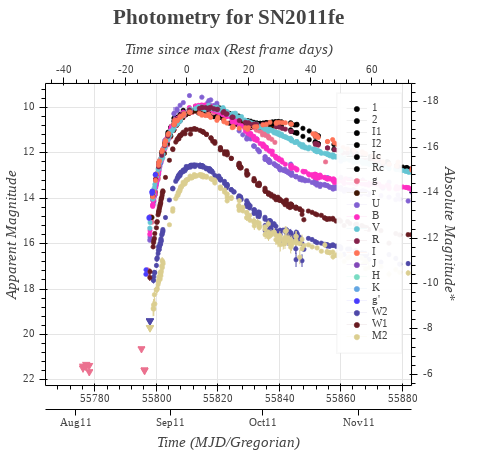
\includegraphics[width=3in,natwidth=6in]{SN2011fe_light_curve.png}};%
%\end{tikzpicture}

%\begin{tabular}{cc}
%A & B
%\includegraphics[width=0.5\textwidth,angle=270]{SN2011fe_55806p2.eps} & B\\
%\end{tabular}
%\end{center}
}


\frame{
\frametitle{Why they matter}
\begin{tabular}{l}
\\
\\
\\
\color{white}\textbf{Brightest standardizable candle}\\
\hspace{2em}Peak luminosity $M_V\sim-19$ ($5\times 10^9$\Lsunp)\\
\hspace{2em}Useful to measure distances to most distant visible galaxies\\
\hspace{2em}Used to measure expansion of the universe\\
\hspace{2em}Used to discover acceleration of expansion (Dark Energy) (Riess et al. 1998, Perlmutter et al. 1999)\\
\\
\\
\\
\color{white}\textbf{Chemical enrichment}\\
\hspace{2em} Each supernova releases $\sim 10^{33}$\;g each of iron, silicon, sulfur (Seitenzahl et al. 2013)\\
\end{tabular}
}

\frame{
\frametitle{What they aren't}
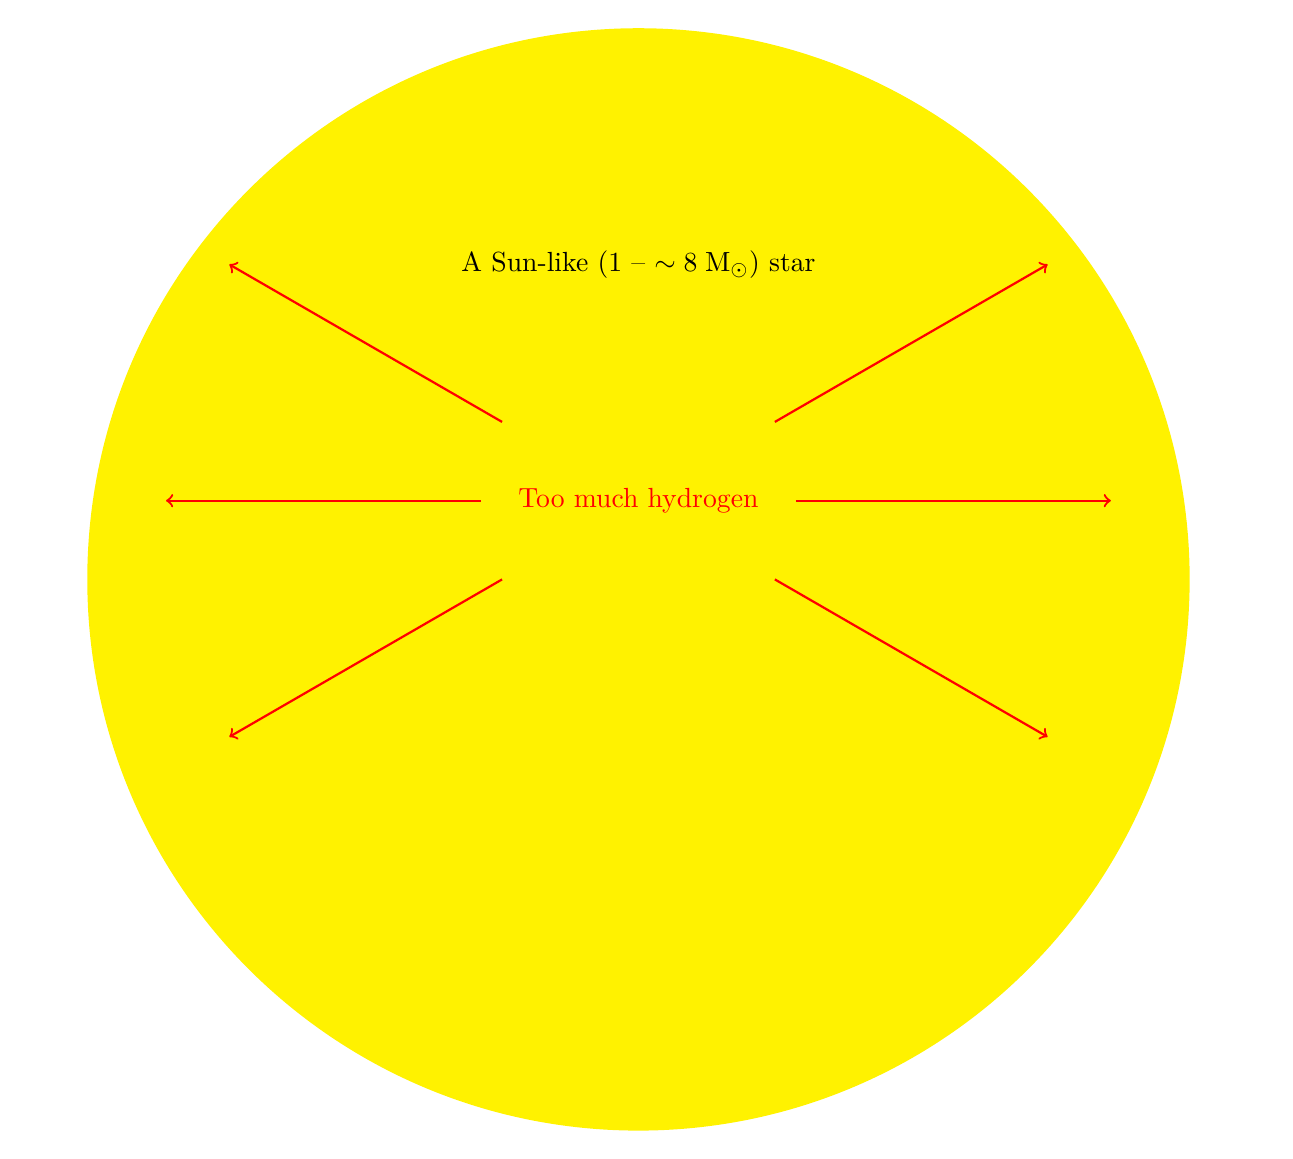
\begin{tikzpicture}
\draw[opacity=0] (0.1,0.1) rectangle (15.8,9);
\fill[yellow] (7.85,2) circle(7);
\draw[black] (7.85,6) node {A Sun-like (1 -- $\sim 8\;\mathrm{M}_\odot$) star};
\draw[red] (7.85,3) node {Too much hydrogen};
\foreach \x in {0,30,-30,150,-150,180}
{
	\draw[red,thick,->] (7.85,3)++(\x:2) -- +(\x:4);
} 
%\draw[white]  (7.85,2) circle(0.07);
\end{tikzpicture}
}

\frame{
\frametitle{But, strip away the hydrogen}
\begin{tikzpicture}
\draw[opacity=0] (0.1,0.1) rectangle (15.8,9);
\fill[white]  (7.85,2) circle(0.07);
\draw[white] (7.85,2.5) node {White dwarf};
\draw[white] (7.85,1.5) node {Former core of sun-like star};
\draw[white] (7.85,1.0) node {About the size of Earth};

\end{tikzpicture}
}

%\frame{
%\frametitle{You're all just a bunch of degenerates}
%\begin{tikzpicture}
%\draw[opacity=0] (0.1,0.1) rectangle (15.8,9);
%\fill[white]  (7.85,6) circle(3);
%\draw[blue,->]  (7.75,6) -- (7.75,8.7);
%\draw[red,<-]  (7.95,6) -- (7.95,8.7);
%\draw[blue]  (7,7.7) node {pressure}; 
%\draw[red]  (8.55,7.1) node {gravity}; 
%\fill[green]  (2.5,6) circle(0.03) ++(0,0.3) node {Electron};
%\draw[green]  (2.5,5) ++(0,0.3) node {Typical gas};
%\node fill[green]  (1.5,5) circle(0.03) draw[green,->] (1.5,5) -- +(15:0.3);
%\foreach \x in {1,...,10}{
%	\coordinate (A) at ($ (2.5,4.3) + 0.5*(rand, rand)$);
%	\fill[green]  (A) circle(0.03);
%	\draw[green,->] (A) -- +(rand*180.0:0.2);
% }
%\draw[green] (2.5,3) ++ (0,0.3) node {Degenerate gas};
%\foreach \x in {1,...,10}{
%	\foreach \y in {1,...,5}{
%		\coordinate (A) at ($ (2.2,2.6) + 0.06*(\x, \y)$);
%		\coordinate (B) at ($ (2.2,2.6) + 0.06*(\x, \y) + (0.030,0.030)$);
%		\fill[green]  (A) circle(0.025);
%		\fill[green]  (B) circle(0.025);
%	}
%}
%\draw[white] (2.5,2) node {Electrons can't fit on top of each other} ++(0,-0.5) node {(limited number of states)};
%
%\end{tikzpicture}
%}

%\frame{
%\frametitle{Who wins?}
%\begin{tikzpicture}
%\draw[opacity=0] (0.1,0.1) rectangle (15.8,9);
%\fill[white]  (7.85,6) circle(3);
%\draw[blue,->]  (7.75,6) -- (7.75,8.7);
%\draw[red,<-]  (7.95,6) -- (7.95,8.7);
%\draw[blue]  (7,7.7) node {pressure}; 
%\draw[red]  (8.55,7.1) node {gravity}; 
%\fill[green]  (2.5,6) circle(0.03) ++(0,0.3) node {Electron};
%\draw[green]  (2.5,5) ++(0,0.3) node {Typical gas};
%%\node fill[green]  (1.5,5) circle(0.03) draw[green,->] (1.5,5) -- +(15:0.3);
%\foreach \x in {1,...,10}{
%	\coordinate (A) at ($ (2.5,4.3) + 0.5*(rand, rand)$);
%	\fill[green]  (A) circle(0.03);
%	\draw[green,->] (A) -- +(rand*180.0:0.2);
% }
%\draw[green] (2.5,3) ++ (0,0.3) node {Degenerate gas};
%\foreach \x in {1,...,10}{
%	\foreach \y in {1,...,5}{
%		\coordinate (A) at ($ (2.2,2.6) + 0.06*(\x, \y)$);
%		\coordinate (B) at ($ (2.2,2.6) + 0.06*(\x, \y) + (0.030,0.030)$);
%		\fill[green]  (A) circle(0.025);
%		\fill[green]  (B) circle(0.025);
%	}
%}
%\draw[white] (2.5,2) node {Electrons can't fit on top of each other} ++(0,-0.5) node {(limited number of states)};

%\draw[white] (12.5,4) node[red,thick] {Gravity} ++(0,-0.5) node[white]{star begins to collapse};
%\draw[white] (12.5,6) node[gray,thick] {Neither} ++(0,-0.5) node[white]{boring};
%\draw[white] (12.5,8.5) node[blue,thick] {Pressure} ++(0,-0.5) node[white]{star expands or explodes};
%\end{tikzpicture}
%}

\frame{
\frametitle{How to explode}
\begin{tabular}{l}
Add mass such that gravity overcomes pressure (how?)\\
At 1.4$\;\mathrm{M}_{\odot}$ gravity starts to win\\
\hspace{2em}Star begins fusing carbon / oxygen $\rightarrow$ (Ne, Mg, Ar, Si, S, Ca)\\
Star detonates (how?), resulting in production of Fe, Co, Ni, lots of energy --- explosion!\\
\end{tabular}
\begin{tikzpicture}
\draw[opacity=0,yellow] (0.1,0.1) rectangle (14.6,7);
\fill[white] (2,3.0) circle(2);
\foreach \x in {1,...,30}{
		\coordinate (A) at ($ (2,5.0) + (-90+rand*15.0:rand*1.5)$);
		\fill[white]  (A) circle(0.03);
}
\foreach \x in {1,...,12}{
		\coordinate (A) at ($ (2,3)+ (\x*360.0/12.0:1.5)$);
		\coordinate (B) at ($ (2,3)+ (\x*360.0/12.0:1.9)$);
		\draw[red,<-] (A) -- (B);
}
\fill[white] (7,3) circle(1.75);
\foreach \x in {1,...,12}{
		\coordinate (A) at ($ (7,3)+ (\x*360.0/12.0:0.3)$);
		\coordinate (B) at ($ (7,3)+ (\x*360.0/12.0:1.5)$);
		\draw[gray,thick,->] (A) -- (B);
}
\fill[white] (12,3) circle(2.5);
\foreach \x in {1,...,12}{
		\coordinate (A) at ($ (12,3)+ (\x*360.0/12.0:0.3)$);
		\coordinate (B) at ($ (12,3)+ (\x*360.0/12.0:2.4)$);
		\draw[blue,thick,->] (A) -- (B);
}
\end{tikzpicture}
}

\frame{
\frametitle{Adding mass}
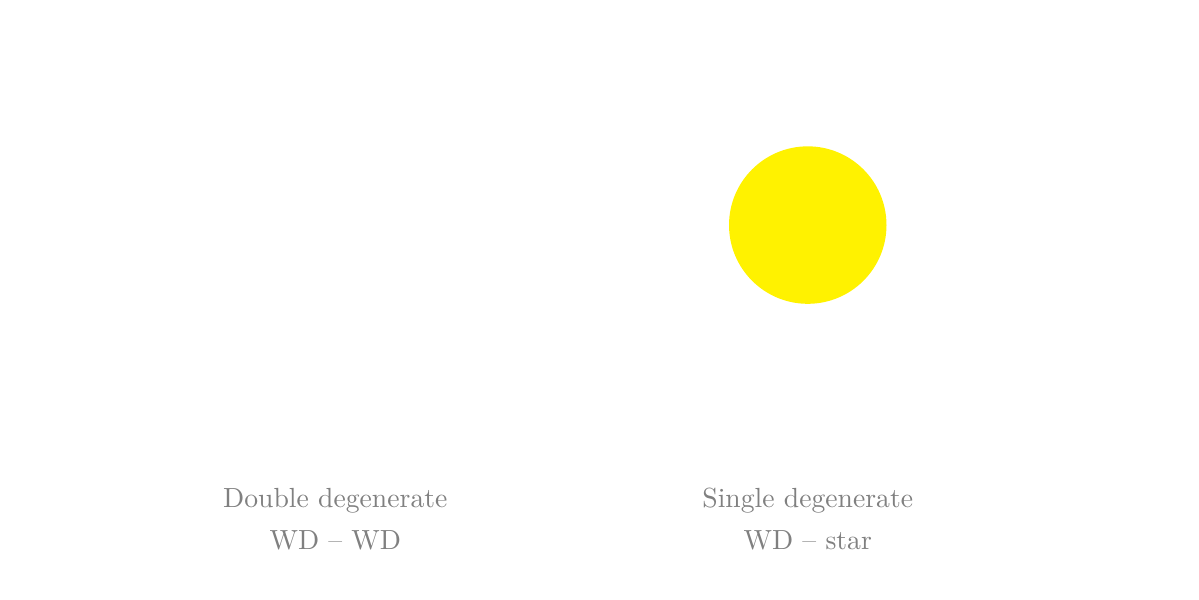
\begin{tikzpicture}
\draw[opacity=0,yellow] (0.1,0.1) rectangle (14.6,7);
\fill[white] (4,4.5) circle(0.05);
\fill[white] (4,1.5) circle(0.05);
\draw[white,->] (5,3)++(-60:1) arc [start angle=-60, end angle=60, radius=1]; 
\draw[white,->] (3,3)++(120:1) arc [start angle=120, end angle=240, radius=1]; 
\draw[gray] (4,1) node {Double degenerate};
\draw[gray] (4,0.5) node {WD -- WD};

\fill[yellow] (10,4.5) circle(1);
\fill[white] (10,1.5) circle(0.05);
\draw[white,->] (11,3)++(-60:1) arc [start angle=-60, end angle=60, radius=1]; 
\draw[white,->] (9,3)++(120:1) arc [start angle=120, end angle=240, radius=1]; 
\draw[gray] (10,1) node {Single degenerate};
\draw[gray] (10,0.5) node {WD -- star};
\end{tikzpicture}
}

\frame{\frametitle{How to tell the two scenarios apart?}
\begin{tabular}{l}
\color{yellow}Have never seen a system prior to explosion\\
\hspace{2em} Need to look for evidence after the fact.\\
\\
\color{white}Single degenerate\\
\hspace{2em} Look for surviving companion\\
\\
\\
\hspace{2em} Look for evidence of interaction with the companion -- e.g. excess UV (Kasen et al. 2010)\\
\\
\\
\color{white}Both\\
\hspace{2em} Look for evidence of material donated by companion\\
\\
\end{tabular}
}

\frame{\frametitle{How to tell the two scenarios apart?}
\begin{tabular}{l}
\color{yellow}Have never seen a system prior to explosion\\
\hspace{2em} Need to look for evidence after the fact.\\
\\
\color{white}Single degenerate\\
\hspace{2em} Look for surviving companion\\
\color{magenta}\hspace{4em} Maybe for Tycho's SN --- c.f. Ruiz-Lapuente et al. (2004)\\
\color{magenta}\hspace{4em} Still not certain --- c.f. Kerzendorf et al. (2018)\\
\hspace{2em} Look for evidence of interaction with the companion -- e.g. excess UV (Kasen et al. 2010)\\
\\
\\
\color{white}Both\\
\hspace{2em} Look for evidence of material donated by companion\\
\\
\end{tabular}
}

\frame{\frametitle{How to tell the two scenarios apart?}
\begin{tabular}{l}
\color{yellow}Have never seen a system prior to explosion\\
\hspace{2em} Need to look for evidence after the fact.\\
\\
\color{white}Single degenerate\\
\hspace{2em} Look for surviving companion\\
\color{magenta}\hspace{4em} Maybe for Tycho's SN --- c.f. Ruiz-Lapuente et al. (2004)\\
\color{magenta}\hspace{4em} Still not certain --- c.f. Kerzendorf et al. (2018)\\
\hspace{2em} Look for evidence of interaction with the companion -- e.g. excess UV (Kasen et al. 2010)\\
\color{magenta}\hspace{4em} c.f. Cao et al. (2015), Marion et al. (2016), Hosseinzadeh et al. (2017),\\
\color{magenta}\hspace{5em} Jiang et al. (2017), Miller et al. (2018)\\
\color{white}Both\\
\hspace{2em} Look for evidence of material donated by companion\\
\\
\end{tabular}
}


\frame{\frametitle{How to tell the two scenarios apart?}
\begin{tabular}{l}
\color{yellow}Have never seen a system prior to explosion\\
\hspace{2em} Need to look for evidence after the fact.\\
\\
\color{white}Single degenerate\\
\hspace{2em} Look for surviving companion\\
\color{magenta}\hspace{4em} Maybe for Tycho's SN --- c.f. Ruiz-Lapuente et al. (2004)\\
\color{magenta}\hspace{4em} Still not certain --- c.f. Kerzendorf et al. (2018)\\
\hspace{2em} Look for evidence of interaction with the companion -- e.g. excess UV (Kasen et al. 2010)\\
\color{magenta}\hspace{4em} c.f. Cao et al. (2015), Marion et al. (2016), Hosseinzadeh et al. (2017),\\
\color{magenta}\hspace{5em} Jiang et al. (2017), Miller et al. (2018)\\
\color{white}Both\\
\hspace{2em} Look for evidence of material donated by companion\\
\color{red}\hspace{4em} Look for it in early spectra\\
\end{tabular}
}

\setbeamertemplate{footline}{\insertsectionhead~\insertpagenumber / 12}

\section{Early spectra \& high-velocity features}
\setcounter{page}{1}
\frame{
\frametitle{Early spectra: SN~2011fe}
\begin{tabular}{l}
\\
First observed within $\sim$1~d after the explosion occurred (Nugent 2011)\\
\\
Nearby (20 million light years / 6.4~Mpc) in Pinwheel galaxy (M101)\\
\\
Peak V brightness of $\sim$10 (bright enough to see in good binoculars)\\
\\
Multiple spectra and photometry (including HST) nearly every day prior to peak brightness\\
\end{tabular}
}

\frame{\frametitle{Early spectra of SN~2011fe}
\begin{tikzpicture}
\draw[opacity=0] (0.1,0.1) rectangle (15.8,9);
\coordinate (A) at ($ (0.1,0.1)+ 0.5*(15.8-11.5,0.5)$);

%\fill [white] (-0.1,-0.1) rectangle (5.1,4.1);
\filldraw [fill=white](A) rectangle +(11.5,8.5) [path picture=
	{
		\node at (path picture bounding box.center) 
		{
			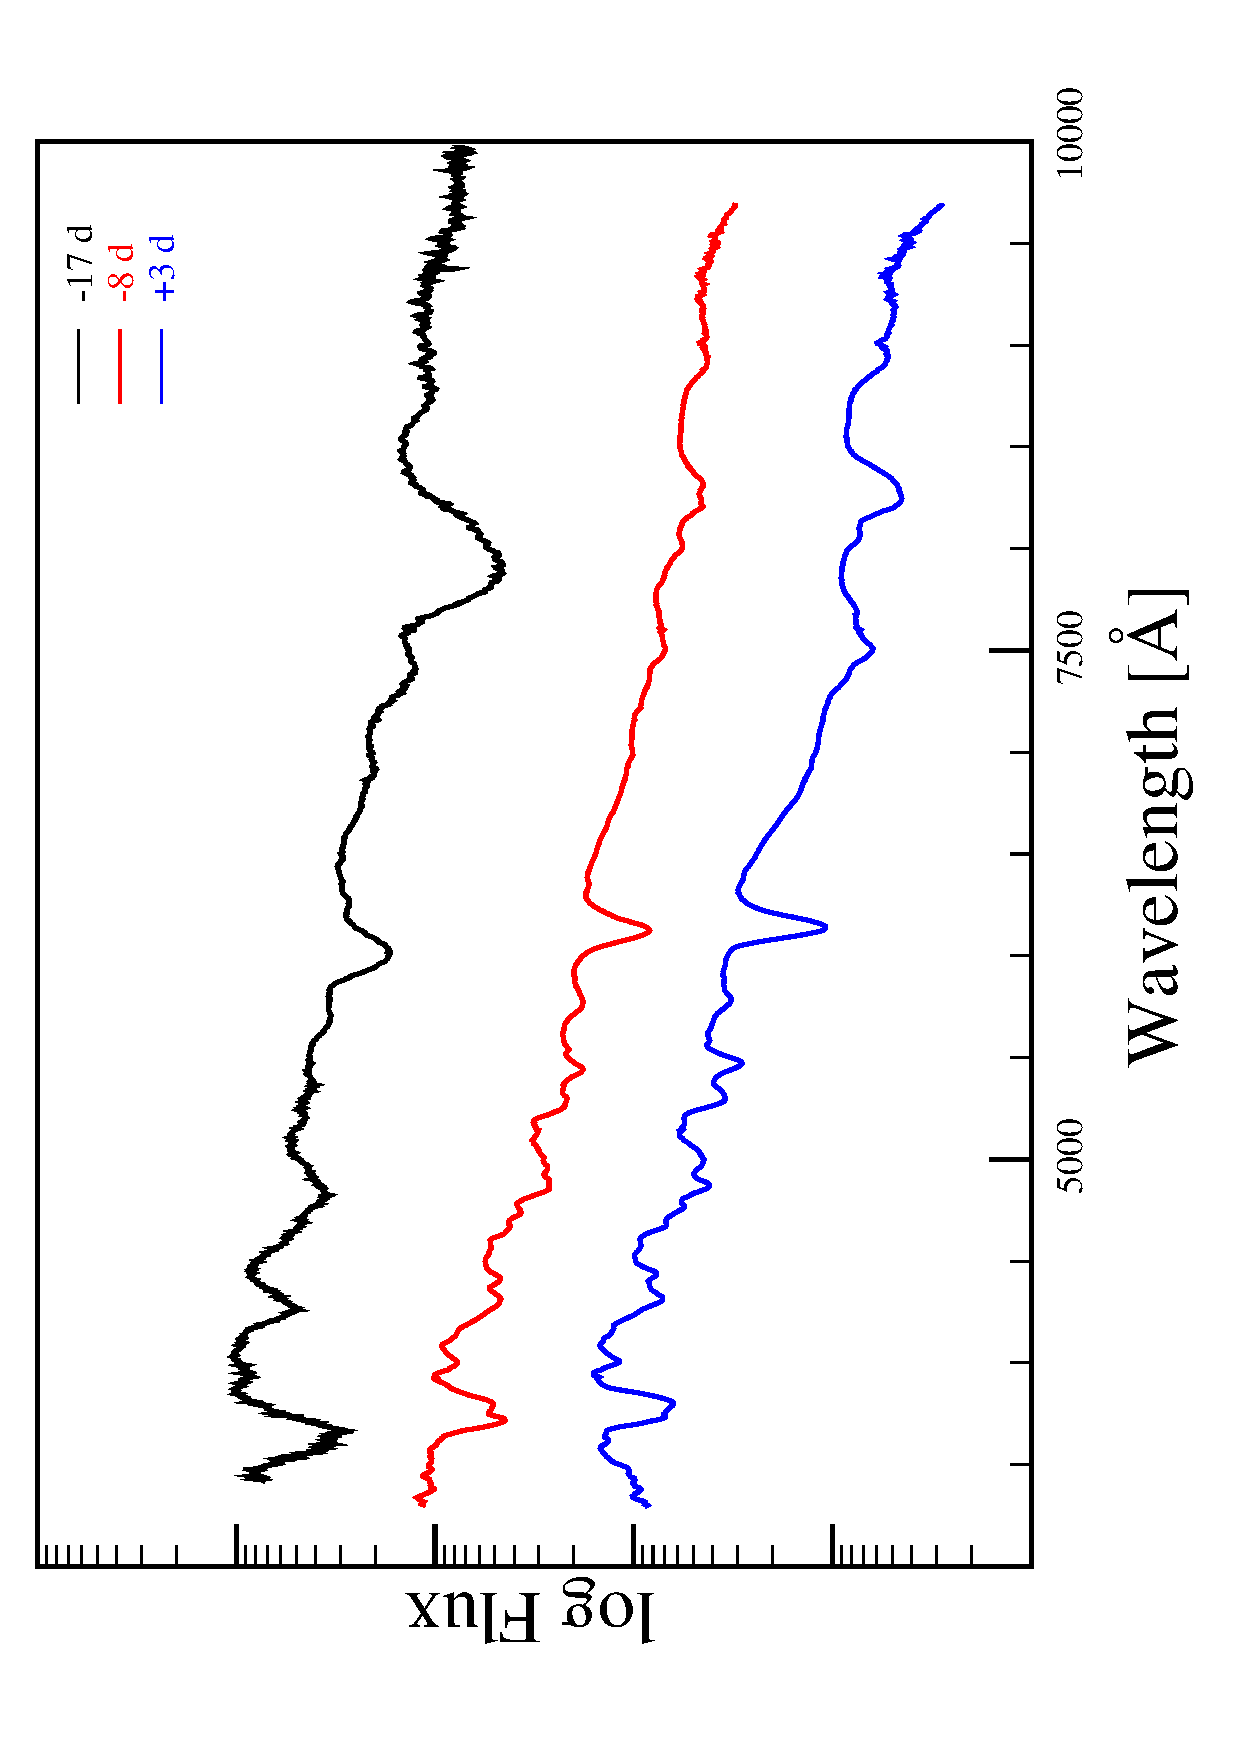
\includegraphics[height=11cm,angle=-90]{early}
		};
	}
];

\fill [fill=gray,opacity=0.25] (9.8,6.8) -- (11.2,6.8) -- (11.5,2.5) -- (10.5,2.5) -- (9.8,6.8);
\draw [gray] (10.5,7) node {Ca};
\fill [fill=red,opacity=0.25] (8.3,6.8) -- (8.8,6.8) -- (8.8,2.5) -- (8.3,2.5) -- (8.3,6.8);
\draw [red] (8.55,7.5) node {No};
\draw [red] (8.55,7) node {H};
\fill [gray,opacity=0.25] (8.2,2.5) -- (7.8,2.5) -- (7.5,6.8) -- (8.2,6.8) -- (8.2,2.5);
\draw [gray] (7.85,7) node {Si};

\end{tikzpicture}
}

\frame{
\frametitle{Evolution of features}
%\begin{center}
\begin{tikzpicture}
\draw[opacity=0] (0.1,0.1) rectangle (15.8,9);
%\fill [white] (-0.1,-0.1) rectangle (5.1,4.1);
\tkzpicmyps{0.1}{0.5}{8.912}{SN2011fe_early_many}
\tkzpich{9.012}{0.5}{6.887}{8.5}{Marion_13_All_Evolution}
\draw[gray] (14.35,1.15) -- +(0,7.60);
\draw[gray,dashed] (14.1,1.15) -- +(0,7.60);
\draw[gray] (12.98,1.15) -- +(0,7.60);
\draw[gray,dashed] (12.85,1.15) -- +(0,7.60);
%\fill[black,opacity=0.4] (9.9,1.15) rectangle +(5.38,3.1);

\draw[white] (4.506,7.75) node {SN 2011fe (Pereira et al. 2013, Mazzali et al. 2014)};
\draw[white,->] (7.9,8.4) -- (8.9,8.40);
\draw[white] (8.9,8.75) node[left] {SN 2009ig (Marion et al. 2013)};

\draw[gray] (0.35,4) node[rotate=90] {Time};
\draw[gray,->] (0.40,4.5) -- +(0,1);

\draw[gray] (15.5,7) node[rotate=-90] {Time};
\draw[gray,->] (15.5,6.5) -- +(0,-1);
\end{tikzpicture}
}

\frame{
\frametitle{Focus on Ca, Si}
%\begin{center}
\begin{tikzpicture}
\draw[opacity=0] (0.1,0.1) rectangle (15.8,9);
%\fill [white] (-0.1,-0.1) rectangle (5.1,4.1);
\begin{scope}[even odd rule]
\clip (2.6,0.5) -- +(0.0,8.0) -- +(4.5,8.0) -- +(4.5,0.0) -- +(0.0,0.0);
\tkzpic{-1.9}{0.5}{9}{8}{Marion_13_Ca_Evolution}
\end{scope}

%\tkzpic{9.1}{0.5}{5}{8}{Marion_13_Ca_Evolution}
\filldraw [fill=white](9.1,0.5) rectangle +(5,8) [path picture=
	{
		\node at (path picture bounding box.center) 
		{
			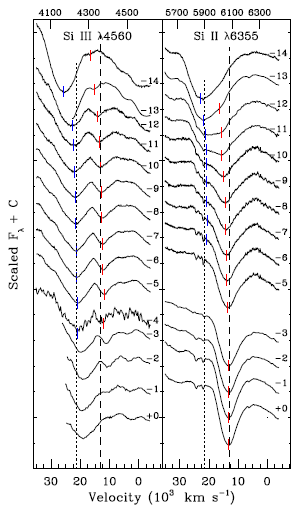
\includegraphics[width=4.5cm]{Marion_13_Si_Evolution}
		};
	}
];
\draw[white] (7.5,8.75) node {SN 2009ig (Marion et al. 2013)};
\end{tikzpicture}
}



\frame{
\frametitle{Two components}
%\begin{center}
\begin{tikzpicture}
\draw[opacity=0] (0.1,0.1) rectangle (15.8,9);
\tkzpic{0.4}{3.5}{15}{4.5}{Childress_Fits}
\draw[white] (7.6,8.5) node {SN 2005cf (Childress et al. 2014)};
\draw[blue] (7.15,5.8) node {HVF};
\draw[magenta] (8.5,6.1) node {PVF};
\draw[magenta] (3.3,6.1) node {PVF};
\draw[green!70!black] (12.4,7.05) node[font=\scriptsize] {Si II};
\draw[blue] (11.75,5.7) node[font=\scriptsize] {HVF};
\draw[magenta] (13.4,6.1) node[font=\scriptsize] {PVF};
\draw[yellow] (7,3.25) node[left] {Photospheric-Velocity Feature (PVF)};
\draw[yellow] (15,3.25) node[left] {High-Velocity Feature (HVF)};
\draw[white] (7.95,2.75) node {HVF occur in nearly all SN~Ia.};
\draw[white] (7.95,2.25) node {Most common in calcium, also found in silicon, oxygen, iron, sulfur.};
\draw[white] (7.95,1.75) node {HVF also exhibit 0.1 -- 1\% polarization == clumpy material};
\draw[white] (7.95,1.25) node { (Wang et al. 2003, Wang \& Wheeler 2008, Patat et al. 2009)};
\draw[white] (7.95,0.5) node {Ca \textsc{II} near-infrared (CaNIR) consistently has HVF, does not suffer from blending.};
\end{tikzpicture}
}


\frame{
\frametitle{Evolution of HVF and PVF}
\begin{tikzpicture}
\draw[opacity=0] (0.1,0.1) rectangle (15.8,9);
\tkzpic{3}{2.5}{10}{8}{Silverman_CaNIR_velocity}
\draw[white] (7.95,2) node {(Silverman et al. 2015)};
\draw[gray] (12.5,9) node[left] {Filled = HVF};
\draw[white] (12.5,8.5) node[left] {\contour{gray}{Hollow}\color{gray}\;= PVF};
\end{tikzpicture}
}

\frame{
\frametitle{Importance of HVF}
\begin{tabular}{l}
Only appear within first few weeks after the explosion.\\
\\
\\
Can give insight into nature of system or cause of the explosion.\\
\\
\\
What is the source of the material for the HVF?\\
\hspace{2em} Related to donor star?\\
\\
\end{tabular}
}

%\frame{
%\frametitle{Evolution of HVF and PVF}
%\begin{tikzpicture}
%\draw[opacity=0] (0.1,0.1) rectangle (15.8,9);
%\tkzpic{1}{2.5}{7}{5.6}{Silverman_CaNIR_velocity}
%\tkzpicmyps{8.0}{2.5}{7.0}{Silverman_Total_pEW}
%\draw[white] (7.95,2) node {(Silverman et al. 2015; Mulligan \& Wheeler 2017)};
%\draw[gray] (7.4,7.5) node[left,font=\scriptsize] {Filled = HVF};
%\draw[white] (7.4,7.0) node[left,font=\scriptsize] {\contour{gray}{Hollow}\color{gray}\;= PVF};
%\draw[black] (12.0,7.3) -- +(0.3,0) node[right,font=\scriptsize] {Average};
%\draw[black,thick] (12.1,7.25) -- (12.2,7.35);
%\draw[black,thick] (12.1,7.35) -- (12.2,7.25);
%\draw[gray] (12.0,7.0) -- +(0.3,0) node[right,font=\scriptsize] {Individual SNe};
%\end{tikzpicture}
%}



%\frame{
%\frametitle{Cause of PVF \& P Cygni emission}
%\begin{center}
%\begin{tikzpicture}
%\draw[opacity=0] (0.1,0.1) rectangle (15.8,9);
%
%\fill[cyan] (4.5,5.0) circle (3);
%\fill[magenta] (4.5,5.0) circle (2.5);
%\fill[white] (4.5,5.0) circle (1.5);
%\draw[yellow, snake it, ->,thick] (6.0,5.0) -- +(4,0);
%\draw[yellow, snake it, ->,thick] (4.5,6.5) -- +(0,2.5);
%\draw[yellow,opacity=0.75, snake it, ->,thick] (4.5,7.0) -- +(4,0);
%\draw[yellow,opacity=0.75, snake it, ->,thick] (6.25,5.0) -- +(60:1);
%\draw[yellow,opacity=0.75, snake it, ->,thick] (6.25,5.0) -- +(-60:1);
%\draw[yellow,opacity=0.75, snake it, ->,thick] (6.75,5.0) -- +(60:1);
%\draw[yellow,opacity=0.75, snake it, ->,thick] (7.0,5.0) -- +(-60:1);
%
%\draw[black] (4.5,5.0) node {Opaque};
%\draw[black] (4.5,5.0)++(-30:1.3) node[left] {Photosphere};
%\draw[black,->] (4.5,5.0)++(-30:1.3) -- +(-30:0.2); 
%\draw[black,opacity=0.7] (4.5,3.25) node {Translucent};
%
%\draw[gray,thick] (1.5,0.80) -- +(6,0);
%\draw[gray,thick] (4.5,0.35) -- +(0,0.9);
%\draw[white,thick] (1.5,0.45) -- +(6,0.8);
%\draw[gray] (4.6,1.05) node [right,font=\tiny] {Velocity +};
%\draw[gray] (4.4,0.45) node [left,font=\tiny] {Velocity -};
%
%
%\draw [green,decorate,decoration={brace,amplitude=10pt}] (4.4,6.5) -- (4.4,7.5);
%\draw [green] (4.0,7.0) node [left] {P Cygni};
%\draw [green,decorate,decoration={brace,amplitude=10pt}] (4.5,5.0)++(20:1.5) -- +(20:1);
%\draw [green] (4.5,5.0)++(35:2.0) node {PVF};
%\draw [green] (7.0,5.75) node {PVF};

%\fill[white] (11,2) rectangle +(4.5,5);
%\draw[gray,dashed] (11.1,4.5) -- +(4.3,0);
%\draw[black,thick] (11.1,4.5) -- +(1,0.0) .. controls +(1,-2.0) .. +(3.5,0) .. controls +(0.45,1.5) .. +(4.3,0);
%\draw[black] (13.15,2.4) node {PVF};
%\draw[black] (14.75,6.2) node {P Cygni};
%\end{tikzpicture}
%}

%\frame{
%\frametitle{Cause of HVF}
%\begin{center}
%\begin{tikzpicture}
%\draw[opacity=0] (0.1,0.1) rectangle (15.8,9);
%\fill[magenta] (4.5,5.0) circle (3.5);
%\fill[cyan] (4.5,5.0) circle (3);
%\fill[magenta] (4.5,5.0) circle (2.5);
%\fill[white] (4.5,5.0) circle (1.5);
%\draw[yellow, snake it, ->,thick] (6.0,5.0) -- +(4,0);
%\draw[yellow, snake it, ->,thick] (4.5,6.5) -- +(0,2.5);
%\draw[yellow,opacity=0.75, snake it, ->,thick] (4.5,7.0) -- +(4,0);
%\draw[yellow,opacity=0.75, snake it, ->,thick] (6.25,5.0) -- +(60:1);
%\draw[yellow,opacity=0.75, snake it, ->,thick] (6.25,5.0) -- +(-60:1);
%\draw[yellow,opacity=0.75, snake it, ->,thick] (6.75,5.0) -- +(60:1);
%\draw[yellow,opacity=0.75, snake it, ->,thick] (7.0,5.0) -- +(-60:1);
%
%\draw[black] (4.5,5.0) node {Opaque};
%\draw[black] (4.5,5.0)++(-30:1.3) node[left] {Photosphere};
%\draw[black,->] (4.5,5.0)++(-30:1.3) -- +(-30:0.2); 
%\draw[black,opacity=0.7] (4.5,3.25) node {Translucent};
%
%\draw[yellow,opacity=0.75, snake it, ->,thick] (4.5,8.25) -- +(4,0);
%\draw[yellow,opacity=0.75, snake it, ->,thick] (7.75,5.0) -- +(-60:1);
%
%\draw [green,decorate,decoration={brace,amplitude=10pt}] (4.4,6.5) -- (4.4,7.5);
%\draw [green] (4.0,7.0) node [left] {P Cygni};
%\draw [green,decorate,decoration={brace,amplitude=10pt}] (4.5,5.0)++(20:1.5) -- +(20:1);
%\draw [green] (4.5,5.0)++(35:2.0) node {PVF};
%\draw [green,decorate,decoration={brace,amplitude=5pt}] (4.5,5.0)++(5:3.0) -- +(5:0.5);
%\draw [green] (4.5,5.0)++(12.5:3.0) node[right] {HVF};
%
%\draw[gray,thick] (1.0,0.80) -- +(7.0,0);
%\draw[gray,thick] (4.5,0.35) -- +(0,0.9);
%\draw[white,thick] (1.0,0.35) -- +(7.0,0.9);
%\draw[gray] (4.6,1.05) node [right,font=\tiny] {Velocity +};
%\draw[gray] (4.4,0.45) node [left,font=\tiny] {Velocity -};
%
%\fill[white] (11,2) rectangle +(4.5,5);
%\draw[gray,dashed] (11.1,4.5) -- +(4.3,0);
%\draw[black,thick] (11.1,4.5) ..controls +(0.5,-2.0) .. +(1,-0.5) .. controls +(1,-2.0) .. +(3.5,0) .. controls +(0.45,1.5) .. +(4.3,0);
%\draw[black] (11.50,2.4) node {HVF};
%\draw[black] (13.15,3.2) node {PVF};
%\draw[black] (14.75,6.2) node {P Cygni};
%\end{tikzpicture}
%}

\frame{
\frametitle{Source of HVF}
\begin{footnotesize}
\begin{tabular}{l}
Clumps of high velocity material ejected from SN\\
\\
\\
\\
Material swept up as SN expands\\
\\
\\
\\
\\
Outer layer of ejecta with different ionization or excitation characteristics\\
\\
\\
Shell of material surrounding SN prior to explosion\\
\\
\end{tabular}
\end{footnotesize}
}

\frame{
\frametitle{Source of HVF}
\begin{footnotesize}
\begin{tabular}{l}
Clumps of high velocity material ejected from SN\\
\color{magenta}\hspace{2em} Explains polarization\\
\color{magenta}\hspace{2em} Likely to be greatly enhanced in freshly synthesized elements\\
\color{magenta}\hspace{2em} No obvious explanation for velocity evolution\\
Material swept up as SN expands\\
\\
\\
\\
\\
Outer layer of ejecta with different ionization or excitation characteristics\\
\\
\\
Shell of material surrounding SN prior to explosion\\
\\
\end{tabular}
\end{footnotesize}
}

\frame{
\frametitle{Source of HVF}
\begin{footnotesize}
\begin{tabular}{l}
Clumps of high velocity material ejected from SN.\\
\color{magenta}\hspace{2em} Explains polarization.\\
\color{magenta}\hspace{2em} Likely to be greatly enhanced in freshly synthesized elements.\\
\color{magenta}\hspace{2em} No obvious explanation for velocity evolution.\\
\sout{Material swept up as SN expands.}\\
\color{magenta}\hspace{2em} Polarization due to instabilities during interaction.\\
\color{magenta}\hspace{2em} Related to wind from progenitor?\\
\color{magenta}\hspace{2em} Outer edge slows as material is swept up.\\
\color{magenta}\hspace{2em} Would result in excess blue light and synchrotron emission that is not observed.\\
Outer layer of ejecta with different ionization or excitation characteristics.\\
\\
\\
Shell of material surrounding SN prior to explosion.\\
\end{tabular}
\end{footnotesize}
}

\frame{
\frametitle{Source of HVF}
\begin{footnotesize}
\begin{tabular}{l}
Clumps of high velocity material ejected from SN.\\
\color{magenta}\hspace{2em} Explains polarization.\\
\color{magenta}\hspace{2em} Likely to be greatly enhanced in freshly synthesized elements.\\
\color{magenta}\hspace{2em} No obvious explanation for velocity evolution.\\
\sout{Material swept up as SN expands.}\\
\color{magenta}\hspace{2em} Polarization due to instabilities during interaction.\\
\color{magenta}\hspace{2em} Related to wind from progenitor?\\
\color{magenta}\hspace{2em} Outer edge slows as material is swept up.\\
\color{magenta}\hspace{2em} Would result in excess blue light and synchrotron emission that is not observed.\\
Outer layer of ejecta with different ionization or excitation characteristics.\\
\color{magenta}\hspace{2em} Some theoretical evidence this may occur (Blondin et al. 2013).\\
\color{magenta}\hspace{2em} May not explain evolution or polarization.\\
Shell of material surrounding SN prior to explosion.\\
\end{tabular}
\end{footnotesize}
}


\frame{
\frametitle{Source of HVF}
\begin{footnotesize}
\begin{tabular}{l}
Clumps of high velocity material ejected from SN.\\
\color{magenta}\hspace{2em} Explains polarization.\\
\color{magenta}\hspace{2em} Likely to be greatly enhanced in freshly synthesized elements.\\
\color{magenta}\hspace{2em} No obvious explanation for velocity evolution.\\
\sout{Material swept up as SN expands.}\\
\color{magenta}\hspace{2em} Polarization due to instabilities during interaction.\\
\color{magenta}\hspace{2em} Related to wind from progenitor?\\
\color{magenta}\hspace{2em} Outer edge slows as material is swept up.\\
\color{magenta}\hspace{2em} Would result in excess blue light and synchrotron emission that is not observed.\\
Outer layer of ejecta with different ionization or excitation characteristics.\\
\color{magenta}\hspace{2em} Some theoretical evidence this may occur (Blondin et al. 2013).\\
\color{magenta}\hspace{2em} May not explain evolution or polarization.\\
Shell of material surrounding SN prior to explosion.\\
\color{magenta}\hspace{2em} Material from donor: evidence of H, He, C / O?\\
\color{magenta}\hspace{2em} He shell relating to deonation?\\ 
\color{magenta}\hspace{4em} Woosley et al. (1980), Nomoto (1982)\\
\color{magenta}\hspace{4.5em} c.f. Shen \& Moore (2014) \& references therein \\
\color{magenta}\hspace{2em} Polarization due to instabilities during interaction.\\
\color{magenta}\hspace{2em} Compact: no ongoing interaction --- no excess emission.\\
\color{magenta}\hspace{2em} Ca content may be sub-Solar -- super-Solar.\\
\color{magenta}\hspace{2em} Velocity evolution through expansion.\\
\end{tabular}
\end{footnotesize}
}

\setbeamertemplate{footline}{\insertsectionhead~\insertpagenumber / 4}

\section{Compact circumstellar shell \& interaction}
\setcounter{page}{1}
\frame{
\frametitle{Schematic of compact shell}
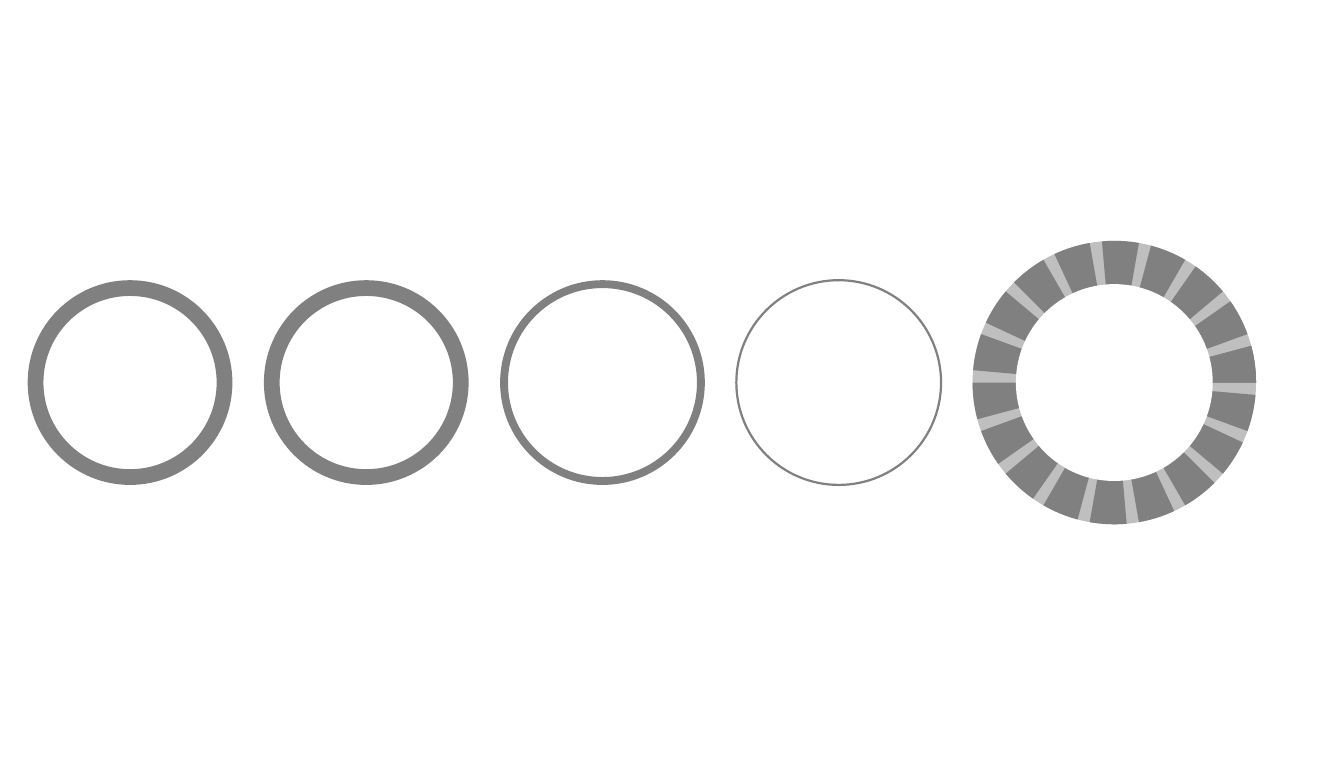
\begin{tikzpicture}
\draw[opacity=0] (0.1,0.1) rectangle (15.8,9);

\fill[white] (1,4.5) circle (0.5);
\draw[gray,line width=0.2cm] (1,4.5) circle (1.2);

\fill[white] (1,4.5)++(3,0) circle (1.0);
\draw[gray,line width=0.2cm] (1,4.5)++(3,0) circle (1.2);

\fill[white] (1,4.5)++(6,0) circle (1.25);
\draw[gray,line width=0.1cm] (1,4.5)++(6,0) circle (1.25);

\fill[white] (1,4.5)++(9,0) circle (1.3);
\draw[gray,thick] (1,4.5)++(9,0) circle (1.3);

\fill[white!50!gray] (1,4.5)++(12.5,0) circle (1.8);
\foreach \x in {0,20,...,360}{
	\fill[gray] (1,4.5)++(12.5,0) -- +(\x:1.8) arc [start angle=\x, end angle=\x+15, radius=1.8] --cycle;
}
\fill[white] (1,4.5)++(12.5,0) circle (1.25);

\end{tikzpicture}
}

\frame{
\frametitle{Hydrodynamics of interaction (1-D)}
\begin{tikzpicture}
\draw[opacity=0] (0.1,0.1) rectangle (15.8,9);
\draw[white] (8.0,8.5) node {FLASH (Fryxell et al. 2000), parameters: mass, radius, density profile of shell.};
\tkzpicmyps{3.55}{1.0}{9.0}{opacity_Si_run57}
\draw[white] (8.0,0.5) node {Mulligan \& Wheeler 2017};
\draw[black] (5.75,6.25) node[font=\small] {Ejecta};
\draw[black] (5.75,5.75) node[font=\small] {(PVF)};
\draw[red] (8.0,5.0) node {Shell};
\draw[red] (8.0,4.5) node {(HVF)};
\draw[red,<-] (6.30,7.00)--+(0.3,0.0) node[right] {Density enhancement};
\draw[red] (6.9,6.50) node[right] {(contact discontinuity)};
\fill[white] (3.6,1.0) rectangle +(0.86,9.0*8.5/11.0);
\draw[black] (3.95,5) node[rotate=90] {Normalized density};
\end{tikzpicture}
}

\frame{
\frametitle{Synthetic spectra using \textsc{syn++}}
\begin{tikzpicture}
\draw[opacity=0] (0.1,0.1) rectangle (15.8,9);
\draw[white] (5.0,8.75) node {\textsc{syn++} (Thomas et al. 2011) modified for arbitrary profile};
\draw[white] (5.0,8.25) node[right] {Allows selection and control of individual ions};
\draw[white] (5.0,7.75) node[right] {specify $T_{\mathrm{PS}}$, $v_{\mathrm{PS}}$, $T_{\mathrm{exc}}$};
\tkzpicmyps{3.1}{1.0}{8.0}{MW18a_Fig_4c}
\draw[white] (8.0,0.5) node {Mulligan \& Wheeler 2018};
\end{tikzpicture}
}

\frame{
\frametitle{Fitting SN~2011fe using \textsc{syn++} (0.005\Msun shell)}
\begin{tikzpicture}
\draw[opacity=0] (0.1,0.1) rectangle (15.8,9);
\begin{scope}[even odd rule]
\clip (2.85,6.42) -- +(0.0,2.58) -- +(3.8,2.58) -- +(3.8,0.0) -- cycle;
\tkzpicmyps{2.85}{6.0}{3.882352941}{MW2_Fig_5a}
\end{scope}
\begin{scope}[even odd rule]
\clip (6.65,6.42) -- +(0.0,2.58) -- +(3.25,2.58) -- +(3.25,0.0) -- cycle;
\tkzpicmyps{6.10}{6.0}{3.882352941}{MW2_Fig_5b}
\end{scope}
\begin{scope}[even odd rule]
\clip (9.90,6.42) -- +(0.0,2.58) -- +(3.25,2.58) -- +(3.25,0.0) -- cycle;
\tkzpicmyps{9.35}{6.0}{3.882352941}{MW2_Fig_5c}
\end{scope}
\begin{scope}[even odd rule]
\clip (2.85,4.22) -- +(0.0,2.2) -- +(3.8,2.2) -- +(3.8,0.0) -- cycle;
\tkzpicmyps{2.85}{3.8}{3.882352941}{MW2_Fig_5d}
\end{scope}
\begin{scope}[even odd rule]
\clip (6.65,4.22) -- +(0.0,2.2) -- +(3.25,2.2) -- +(3.25,0.0) -- cycle;
\tkzpicmyps{6.10}{3.8}{3.882352941}{MW2_Fig_5e}
\end{scope}
\begin{scope}[even odd rule]
\clip (9.90,4.22) -- +(0.0,2.2) -- +(3.25,2.2) -- +(3.25,0.0) -- cycle;
\tkzpicmyps{9.35}{3.8}{3.882352941}{MW2_Fig_5f}
\end{scope}
\begin{scope}[even odd rule]
\clip (2.85,1.6) -- +(0.0,2.62) -- +(3.8,2.62) -- +(3.8,0.0) -- cycle;
\tkzpicmyps{2.85}{1.6}{3.882352941}{MW2_Fig_5g}
\end{scope}
\begin{scope}[even odd rule]
\clip (6.65,1.6) -- +(0.0,2.62) -- +(3.25,2.62) -- +(3.25,0.0) -- cycle;
\tkzpicmyps{6.10}{1.6}{3.882352941}{MW2_Fig_5h}
\end{scope}
\begin{scope}[even odd rule]
\clip (9.90,1.6) -- +(0.0,2.62) -- +(3.25,2.62) -- +(3.25,0.0) -- cycle;
\tkzpicmyps{9.35}{1.6}{3.882352941}{MW2_Fig_5i}
\end{scope}
\draw[white] (8.0,0.5) node {Mulligan \& Wheeler (2018)};
\draw[black] (3.45,8.25) node[right] {1.16~d};
\draw[black] (6.65,6.62) node[right] {1.6~d};
\draw[black] (9.90,6.62) node[right] {2.56~d};
\draw[black] (3.45,4.42) node[right] {2.6~d};
\draw[black] (6.65,4.42) node[right] {4.4~d};
\draw[black] (9.90,4.42) node[right] {7.5~d};
\draw[black] (3.45,2.22) node[right] {10.7~d};
\draw[black] (6.65,2.22) node[right] {14.7~d};
\draw[black] (9.90,2.22) node[right] {17.7~d};
\end{tikzpicture}
}

%\frame{
%\frametitle{Fitting SN~201fe using \textsc{syn++}: $T_{\mathrm{eff}}$, $v_{\mathrm{ps}}$, Ca \textsc{II} optical depth }
%\begin{tikzpicture}
%\draw[opacity=0] (0.1,0.1) rectangle (15.8,9);
%\tkzpicmyps{0.5}{3.0}{5}{MW2_Fig_1}
%\tkzpicmyps{5.5}{3.0}{5}{MW2_Fig_2}
%\tkzpicmyps{10.5}{3.0}{5}{MW2_Fig_3}
%\fill[white] (10.5,3.0) rectangle +(0.5,5*8.5/11);
%\draw[black] (10.75,3+5*8.5/11*0.5) node[rotate=90,font=\tiny] {log Optical Depth};
%\draw[white] (8,1.0) node {Mulligan \& Wheeler 2018};
%\end{tikzpicture}
%}

\setbeamertemplate{footline}{\insertsectionhead~\insertpagenumber / 7}

\section{The composition of the shell}
\setcounter{page}{1}
\frame{
\frametitle{Identifying the composition of the shell}
\begin{tikzpicture}
\draw[opacity=0] (0.1,0.1) rectangle (15.8,9);
\tkzpicmyps{1.75}{4.0}{6}{abundance_Solar_mass}
\tkzpicmyps{8.25}{4.0}{6}{abundance_Solar_velocity}
\draw[white] (8,3.75) node {Use \textsc{tardis} (Kerzendorf \& Sims 2013) to generate spectra from models.};
\draw[white] (8,3.25) node {NLTE, requires explicit specification of composition.};
\draw[white] (8,2.75) node {Ejecta: Gamezo et al. (2005) + Seitenzahl et al. (2013) N100};
\draw[white] (8,2.25) node {Shell substrate: hydrogen, helium, or carbon/oxygen};
\draw[white] (8,1.75) node {Shell Ca abundance: 0 -- 7~dex relative to Solar};
\draw[white] (8,1.25) node {Also: Shen \& Moore (2014) helium envelope detonations}; 
\draw[white] (8,0.75) node {Mulligan, Zhang, \& Wheeler (in prep.)};
\end{tikzpicture}
}


\frame{
\frametitle{Shen \& Moore (2014) envelopes}
\begin{tikzpicture}
\draw[opacity=0] (0.1,0.1) rectangle (15.8,9);
\draw[white] (8.0,8.0) node {0.005, 0.01, 0.02\Msun -- range of expected shell mass \& contains calcium};
\tkzpicmyps{0.5}{3.5}{5}{d02_Seit+0p0_Shen-XpXXX}
\tkzpicmyps{5.5}{3.5}{5}{d05_Seit+0p0_Shen-XpXXX}
\tkzpicmyps{10.5}{3.5}{5}{d09_Seit+0p0_Shen-XpXXX}
\draw[white] (3.0,3.25) node {2~d};
\draw[white] (8.0,3.25) node {5~d};
\draw[white] (13.0,3.25) node {9~d};
\draw[white] (8,2.5) node {Selected envelopes do very poor job at 2 \& 5~d};
\draw[white] (8,2.0) node {Tighly constrained envelope near 0.008\Msun may generate accurate spectrum};
\draw[white] (8,1.5) node {No explanation why mass would be 0.008\Msun };
\draw[white] (8,0.75) node {Mulligan, Zhang, \& Wheeler (in prep.)};
\end{tikzpicture}
}

\frame{
\frametitle{Effect of the substrate? }
\begin{tikzpicture}
\draw[opacity=0] (0.1,0.1) rectangle (15.8,9);
\tkzpicmyps{0.5}{3.0}{5}{d02_Seit+0p0_H-Solar+XpX}
\tkzpicmyps{5.5}{3.0}{5}{d02_Seit+0p0_He-Solar+XpX}
\tkzpicmyps{10.5}{3.0}{5}{d02_Seit+0p0_CO-Solar+XpX}
\draw[white] (3.0,3.25) node {H (2~d)};
\draw[white] (8.0,3.25) node {He (2~d)};
\draw[white] (13.0,3.25) node {C/O (2~d)};
\draw[white] (8,2.0) node {Substrate does not appear in the spectrum};
\draw[white] (8,0.5) node {Mulligan, Zhang, \& Wheeler (in prep.)};
\end{tikzpicture}
}

\frame{
\frametitle{As time goes by}
\begin{tikzpicture}
\draw[opacity=0] (0.1,0.1) rectangle (15.8,9);
\tkzpicmyps{0.5}{3.0}{5}{d02_Seit+0p0_H-Solar+XpX_CaNIR}
\tkzpicmyps{5.5}{3.0}{5}{d05_Seit+0p0_H-Solar+XpX_CaNIR}
\tkzpicmyps{10.5}{3.0}{5}{d09_Seit+0p0_H-Solar+XpX_CaNIR}
\draw[white] (3.0,2.75) node {2~d};
\draw[white] (8.0,2.75) node {5~d};
\draw[white] (13.0,2.75) node {9~d};
\draw[white] (8,2.0) node {Vary calcium abundance relative to Solar by factor of 1 -- $10^4$ (0 -- 4~dex).};
\draw[white] (8,0.5) node {Mulligan, Zhang, \& Wheeler (in prep.)};
\end{tikzpicture}
}


\frame{
\frametitle{Calcium yield in the supernova}
\begin{tikzpicture}
\draw[opacity=0] (0.1,0.1) rectangle (15.8,9);
\tkzpicmyps{0.5}{3.0}{5}{d02_Seit+XpX_H-Solar+0p0_CaNIR}
\tkzpicmyps{5.5}{3.0}{5}{d05_Seit+XpX_H-Solar+0p0_CaNIR}
\tkzpicmyps{10.5}{3.0}{5}{d09_Seit+XpX_H-Solar+0p0_CaNIR}
\draw[white] (3.0,2.75) node {2~d};
\draw[white] (8.0,2.75) node {5~d};
\draw[white] (13.0,2.75) node {9~d};
\draw[white] (8,2.0) node {Vary calcium yield in ejecta relative to Seitenzahl (2013) N100 by $10^{-5}$ -- 1 (-5 -- 0~dex).};
\draw[white] (8,1.5) node {Need slower photosphere or different structure of calcium in ejecta?};
\draw[white] (8,0.5) node {Mulligan, Zhang, \& Wheeler (in prep.)};
\end{tikzpicture}
}


\frame{
\frametitle{``Best'' fit}
\begin{tikzpicture}
\draw[opacity=0] (0.1,0.1) rectangle (15.8,9);
\tkzpicmyps{0.5}{3.0}{5}{d02_Seit-best_H-Solar+best_CaNIR}
\tkzpicmyps{5.5}{3.0}{5}{d05_Seit-best_H-Solar+best_CaNIR}
\tkzpicmyps{10.5}{3.0}{5}{d09_Seit-best_H-Solar+best_CaNIR}
\draw[white] (3.0,2.75) node {2~d};
\draw[white] (8.0,2.75) node {5~d};
\draw[white] (13.0,2.75) node {9~d};
\draw[white] (8,2.0) node {Need to crank up calcium abundance in shell with time?};
\draw[white] (8,0.75) node {Mulligan, Zhang, \& Wheeler (in prep.)};
\end{tikzpicture}
}

\frame{
\frametitle{Findings \& Implications}
\begin{footnotesize}
\begin{tabular}{l}
\color{white}Shell model does OK job of generating HVF\\
\hspace{2em} Velocity of HVF at 5+ days better explained by shell with mass 0.005\Msunp.\\
\hspace{2em} Shallow HVF, too blue\\
\hspace{4em} Gradient in calcium abundance in the shell?\\
\hspace{2em} HVF insufficiently distinct.\\
\hspace{4em} Too much calcium in ejecta at high velocity?\\
\color{white}Silicon or other HVF?\\
\color{white}Solar -- super-Solar abundance of calcium\\
\hspace{2em} Where does so much calcium come from?\\
\hspace{4em} Is \textsc{tardis} getting the ion populations right?\\
\hspace{2em} Why are HVF so common?\\
\hspace{4em} If SN~Ia come from old populations, expect sub-solar calcium.\\
\hspace{2em} No HVF besides calcium.\\
\hspace{2em} Suggests need for super-Solar content to get HVF.\\
\color{white}Substrate does not appear in spectra\\
\hspace{2em} Will it be ever be visible?\\
\color{white} Shen \& Moore (2013) envelopes do not produce spectra that look anything like observed SN~Ia.\\
\hspace{2em} 0.008\Msun envelope?
\end{tabular}
\end{footnotesize}
}

\setbeamertemplate{footline}{\insertsectionhead~\insertpagenumber / 3}

\section{Outstanding questions \& summary}
\setcounter{page}{1}
\frame{
\frametitle{Questions}
\begin{tabular}{l}
\color{white}Why does the calcium content need to increase with time?\\
\hspace{2em} Artificial way of cranking up Ca \textsc{II} abundance.\\
\hspace{2em} Physics missing in \textsc{tardis}?\\
\hspace{2em} Evidence of sweeping up material instead of expanding shell?\\
\hspace{4em} If so, why is there no light signature?\\
\color{white}Is the 0.008\Msun Shen \& Moore (2013) type helium envelope physically motivated?\\
\hspace{2em} There is no known reason why one mass of envelope is preferred over any other.\\
\color{white}What is the light signature of the shell during shock breakout?\\
\hspace{2em} How long is it visible?\\
\end{tabular}
}

\frame{
\frametitle{Next}
\begin{tikzpicture}
\draw[opacity=0] (0.1,0.1) rectangle (15.8,9);
\draw[white] (8,4.5) node[font=\Huge] {?};
\draw[white] (8,3.0) node {University level teaching};
\end{tikzpicture}
}

\frame{
\frametitle{Summary}
\begin{tabular}{l}
\color{white}HVF in SN~Ia\\
\hspace{1.5em} $\sim$30,000 (1~d) -- $\sim$20,000\kms (peak brightness)\\
\hspace{1.5em} Polarized = clumpy.\\
\hspace{1.5em} Disappear around the time of peak brightness.\\
\hspace{1.5em} Distinct from PVF.\\
\\
\color{white}Interaction between SN \& compact, circumstellar shell:\\
\hspace{1.5em} Interaction done in seconds -- no excess radiation at epochs when SNe are observed.\\
\hspace{1.5em} Velocity of contact discontinuity $\sim$15 -- 25,000\kmsp.\\
\hspace{1.5em} Maximum velocity of shell $\sim$ 100,000\kmsp.\\
\hspace{1.5em} Mass of $\sim$0.01\Msun; 0.005\Msun explains velocity of HVF at $>$ 1 week after explosion.\\
\hspace{1.5em} Requires Solar -- super-Solar calcium abundance?\\
\hspace{1.5em} Requires super-Solar silicon abundance?\\
\hspace{1.5em} Substrate unclear -- won't show up in spectra.\\
\hspace{1.5em} If shell is associated with helium envelope \& detonation, needs to be narrowly defined mass.\\
\hspace{1.5em} Still not clear if shell model explains HVF.\\
\end{tabular}
}


\section*{bibliography}


\end{document}

